% Copyright 2004 by Till Tantau <tantau@users.sourceforge.net>.
%
% In principle, this file can be redistributed and/or modified under
% the terms of the GNU Public License, version 2.
%
% However, this file is supposed to be a template to be modified
% for your own needs. For this reason, if you use this file as a
% template and not specifically distribute it as part of a another
% package/program, I grant the extra permission to freely copy and
% modify this file as you see fit and even to delete this copyright
% notice. 

\documentclass{beamer}

% There are many different themes available for Beamer. A comprehensive
% list with examples is given here:
% http://deic.uab.es/~iblanes/beamer_gallery/index_by_theme.html
% You can uncomment the themes below if you would like to use a different
% one:
%\usetheme{AnnArbor}
%\usetheme{Antibes}
%\usetheme{Bergen}
%\usetheme{Berkeley}
%\usetheme{Berlin}
%\usetheme{Boadilla}
%\usetheme{boxes}
%\usetheme{CambridgeUS}
%\usetheme{Copenhagen}
%\usetheme{Darmstadt}
%\usetheme{default}
%\usetheme{Frankfurt}
%\usetheme{Goettingen}
%\usetheme{Hannover}
%\usetheme{Ilmenau}
%\usetheme{JuanLesPins}
%\usetheme{Luebeck}
\usetheme{Madrid}
%\usetheme{Malmoe}
%\usetheme{Marburg}
%\usetheme{Montpellier}
%\usetheme{PaloAlto}
%\usetheme{Pittsburgh}
%\usetheme{Rochester}
%\usetheme{Singapore}
%\usetheme{Szeged}
%\usetheme{Warsaw}

\usepackage{booktabs}
\usepackage{siunitx}
\usepackage{graphicx} 
\usepackage{amsmath}
\usepackage{caption}
\usepackage[italian]{babel}
%\usepackage[utf8]{inputenc

\title{Amplificatore Operazionale II}

% A subtitle is optional and this may be deleted
\subtitle{Studio del comportamento di un op-amp reale in amplificazione di segnali periodici}

\author{S.~Bottaro\inst{1} \and L.M.~Perrone\inst{1}}
% - Give the names in the same order as the appear in the paper.
% - Use the \inst{?} command only if the authors have different
%   affiliation.

\institute[Unipi] % (optional, but mostly needed)
{
  \inst{1}%
  Dipartimento di Fisica\\
  Universita' di Pisa
}
% - Use the \inst command only if there are several affiliations.
% - Keep it simple, no one is interested in your street address.

\date{Recitation - Week03, 2015}
% - Either use conference name or its abbreviation.
% - Not really informative to the audience, more for people (including
%   yourself) who are reading the slides online

%\subject{Theoretical Computer Science}
% This is only inserted into the PDF information catalog. Can be left
% out. 

% If you have a file called "university-logo-filename.xxx", where xxx
% is a graphic format that can be processed by latex or pdflatex,
% resp., then you can add a logo as follows:

% \pgfdeclareimage[height=0.5cm]{university-logo}{university-logo-filename}
% \logo{\pgfuseimage{university-logo}}

% Delete this, if you do not want the table of contents to pop up at
% the beginning of each subsection:
\AtBeginSubsection[]
{
  \begin{frame}<beamer>{Outline}
    \tableofcontents[currentsection,currentsubsection]
  \end{frame}
}

% Let's get started
\begin{document}

\begin{frame}
  \titlepage
\end{frame}

\begin{frame}{Outline}
  \tableofcontents
  % You might wish to add the option [pausesections]
\end{frame}

% Section and subsections will appear in the presentation overview
% and table of contents.
\section{Simulazione con TINA}


\begin{frame}{First Slide Title}{Optional Subtitle}
  \begin{itemize}
  \item {
    My first point.
  }
  \item {
    My second point.
  }
  \end{itemize}
\end{frame}

\subsection{Second Subsection}

% You can reveal the parts of a slide one at a time
% with the \pause command:
\begin{frame}{Second Slide Title}
  \begin{itemize}
  \item {
    First item.
    \pause % The slide will pause after showing the first item
  }
  \item {   
    Second item.
  }
  % You can also specify when the content should appear
  % by using <n->:
  \item<3-> {
    Third item.
  }
  \item<4-> {
    Fourth item.
  }
  % or you can use the \uncover command to reveal general
  % content (not just \items):
  \end{itemize}
\end{frame}


\begin{frame}{Blocks}
\begin{block}{Block Title}
You can also highlight sections of your presentation in a block, with it's own title
\end{block}
\begin{theorem}
There are separate environments for theorems, examples, definitions and proofs.
\end{theorem}
\begin{example}
Here is an example of an example block.
\end{example}
\end{frame}


\begin{frame}{Assegnazione delle incertezze}
\begin{itemize}
\item Errore sul \textsc{gain} $ \approx $ (errore di acquisizione DAQ $ \oplus $ errore del generatore di funzioni).

\begin{definition}
$ \Delta _{DAQ} = 5 mV$ ; $ \Delta _{GEN} = max\{1 \% V_{PP}, 2\si{mV}rms\}$
\end{definition}

\begin{example}
$\Delta G = G * \sqrt{(\frac{max\{1 \% V_{PP}, 2\si{mV}rms\}}{V_{PP}})^2 + (\frac{5\si{mV}}{V_{out}})^2}$
\end{example}


\item Errore sulle \textit{frequenze} $ \approx $ errore del generatore di funzioni).

\begin{definition}
$ \Delta _{GEN} = max\{5E-5 \% f, 40\si{mHz}\}$
\end{definition}

\begin{example}
$\Delta f = max\{5E-5 \% f, 40\si{mHz}\} $
\end{example}

\end{itemize}
\end{frame}

\begin{frame}

{
\centering
\begin{tabular}{|c|c|}
\hline 
Grandezza & Risultati prima simulazione TINA\\ 
\hline 
$R_1$ (k$\Omega$)& 1.03  \\ 
\hline 
$R_2$ (k$\Omega$) & 99.8 \\ 
\hline 
Second Pole (MHz) & 1 \\ 
\hline
Open loop gain & 200k\\
\hline 
 
$f_T (kHz)$ & 10.3 \\ 
\hline 
$f_{\frac{1}{2}} (kHz)$ & 17.8 \\ 
\hline 
Max Gain & 97.8 \\ 
\hline 
\end{tabular}\\
 
 \begin{tabular}{|c|c|}
 \hline 
 Grandezza & Dati sperimentali \\ 
 \hline 
 $f_T (kHz)$ & 8.77 $\pm$ 0.09 \\ 
 \hline 
 $f_{\frac{1}{2}} (kHz)$ & 15.14 $\pm$ 0.16 \\ 
 \hline 
 Max Gain & 97.8 $\pm$ 0.1 \\ 
 \hline 
 \end{tabular}
 
} 
 
\end{frame}

\begin{frame}
\begin{figure}
\centering
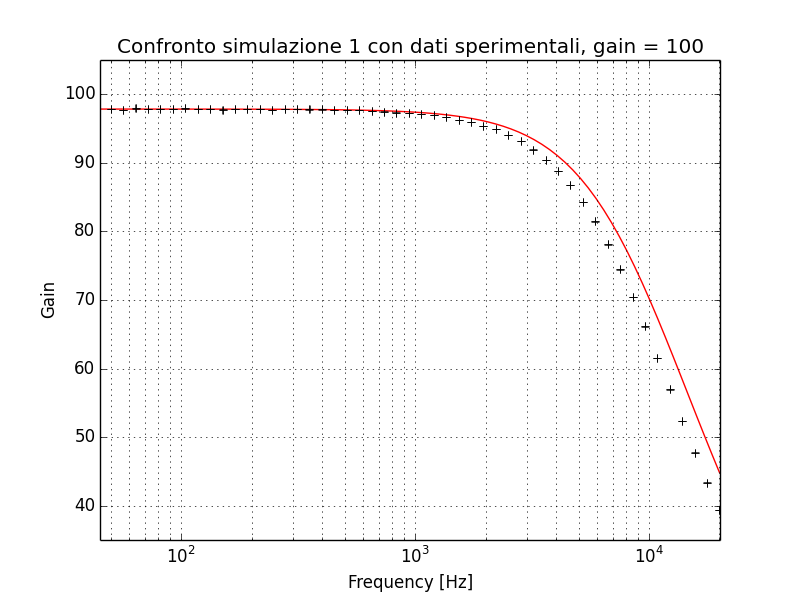
\includegraphics[width=0.9\linewidth]{./es8comparisons_nonsim}
\caption{Simulazione TINA (1) e dati sperimentali - Comparison}
\label{fig:es8comparisons_nonsim}
\end{figure}

\end{frame}

\begin{frame}

{
\centering
\begin{tabular}{|c|c|}
\hline 
Grandezza & Risultati seconda simulazione TINA\\ 
\hline 
$R_1$ (k$\Omega$)& 1.03  \\ 
\hline 
$R_2$ (k$\Omega$) & 99.8 \\ 
\hline 
Second Pole (MHz) & 1 \\ 
\hline
Open loop gain & 171k\\
\hline 
$f_T (kHz)$ & 8.77 \\ 
\hline 
$f_{\frac{1}{2}} (kHz)$ & 15.2 \\ 
\hline 
Max Gain & 97.84 \\ 
\hline 

\end{tabular}


\begin{tabular}{|c|c|}
\hline 
Grandezza & Dati sperimentali \\ 
\hline 
$f_T (kHz)$ & 8.77 $\pm$ 0.09 \\ 
\hline 
$f_{\frac{1}{2}} (kHz)$ & 15.14 $\pm$ 0.16 \\ 
\hline 
Max Gain & 97.8 $\pm$ 0.1 \\ 
\hline 
\end{tabular} 
 
}
\end{frame}

\begin{frame}
\begin{figure}
\centering
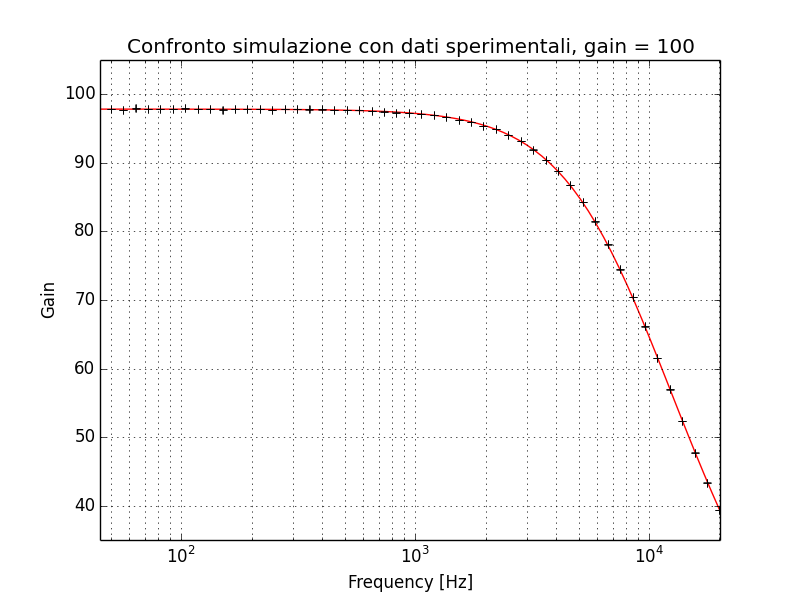
\includegraphics[width=0.9\linewidth]{./es8comparisons}
\caption{Simulazione TINA (2) e dati sperimentali - comparison}
\label{fig:es8comparisons}
\end{figure}

\end{frame}

\section{Analisi in frequenza con generatore esterno}

\subsection{G-100}

\begin{frame}

{
\centering
\begin{tabular}{|c|c|}
\hline  &  \textbf{Dati sperimentali G100} \\ 
\hline $R_1$ (k$\Omega$) &  1.03 $\pm$ 0.8 \% \\ 
\hline $R_2$ (k$\Omega$) & 99.8 $\pm$ 0.8 \%  \\ 
\hline Second Pole (MHz) & 1   \\ 
\hline Open loop gain & 200k    \\ 
\hline $V_{PP}$ & $100  \pm 3 \si{mV} $ \\ 
\hline G &  $G_{exp}(G_{exp}^{\beta})  = 97 \pm 1 (97) \, G_{meas} = 97 \pm 2 $ \\ 
\hline $f_T (kHz)$ &  8.77 $\pm$ 0.09 \\
\hline $f_{\frac{1}{2}} (kHz)$ &  15.14 $\pm$ 0.16 \\
\hline $G*f_{T}$ \si{kHz} & $ 850 \pm 30 $\\
\hline
\end{tabular} 

}
\end{frame}

\begin{frame}
\begin{figure}
\centering
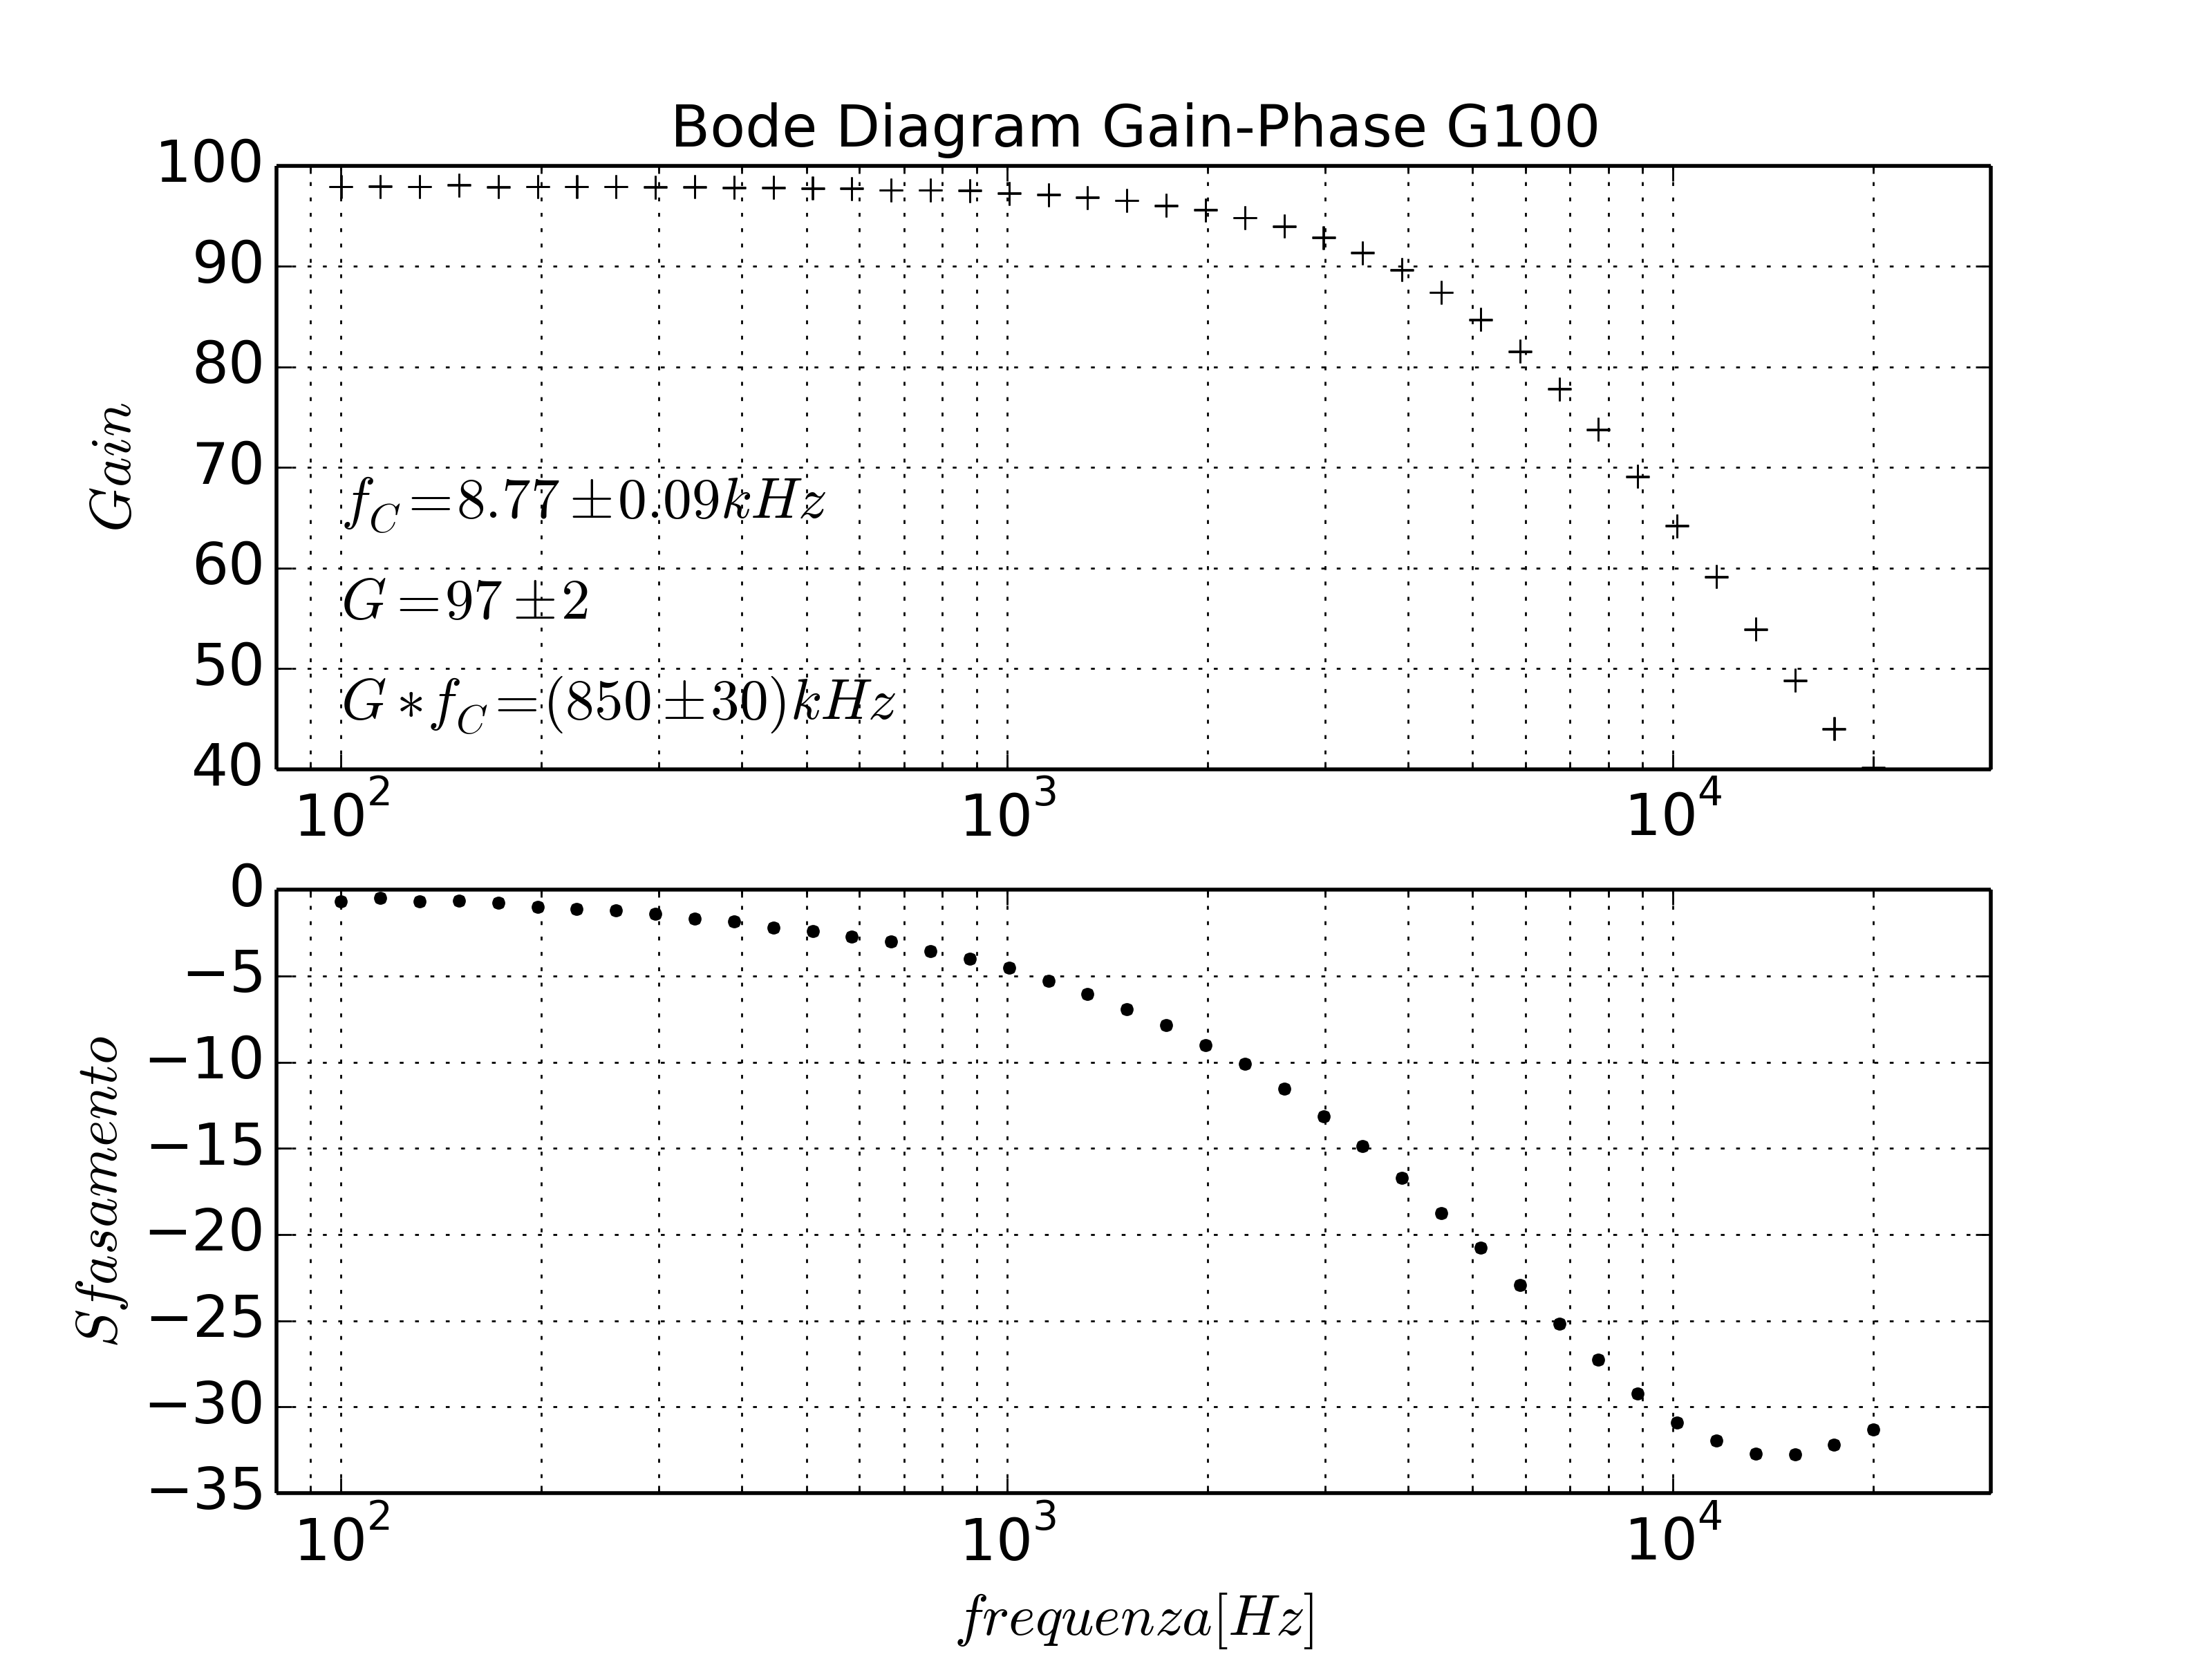
\includegraphics[width=1\linewidth]{./es_8_bode_diag}
\caption{Diagramma di Bode - Gain 100}
\label{fig:es_8_bode_diag}
\end{figure}

\end{frame}

\begin{frame}

{
\centering
\begin{tabular}{|c|c|}
\hline  &  \textbf{Dati sperimentali G300} \\ 
\hline $R_1$  &  98 \si{Ohm} + 1.03 \si{kOhm} ($\pm$ 0.8 \%) \\ 
\hline $R_2$ & 353 \si{kOhm} $\pm$ 0.8 \%  \\ 
\hline $V_{PP}$ & $50  \pm 3 \si{mV} $ \\ 
\hline $V_{OFF} preset$ & $ -46  \si{mV} $ \\
\hline G &  $G_{exp}  = 312 \pm 9  \, G_{meas} = 310 \pm 2 $ \\ 
\hline $f_T (kHz)$ &  2.7 $\pm$ 0.1 \\
\hline $G*f_{T}$ \si{kHz} & $ 840 \pm 40 $\\
\hline
\end{tabular}
 
}

\end{frame}

\begin{frame}
\begin{figure}
\centering
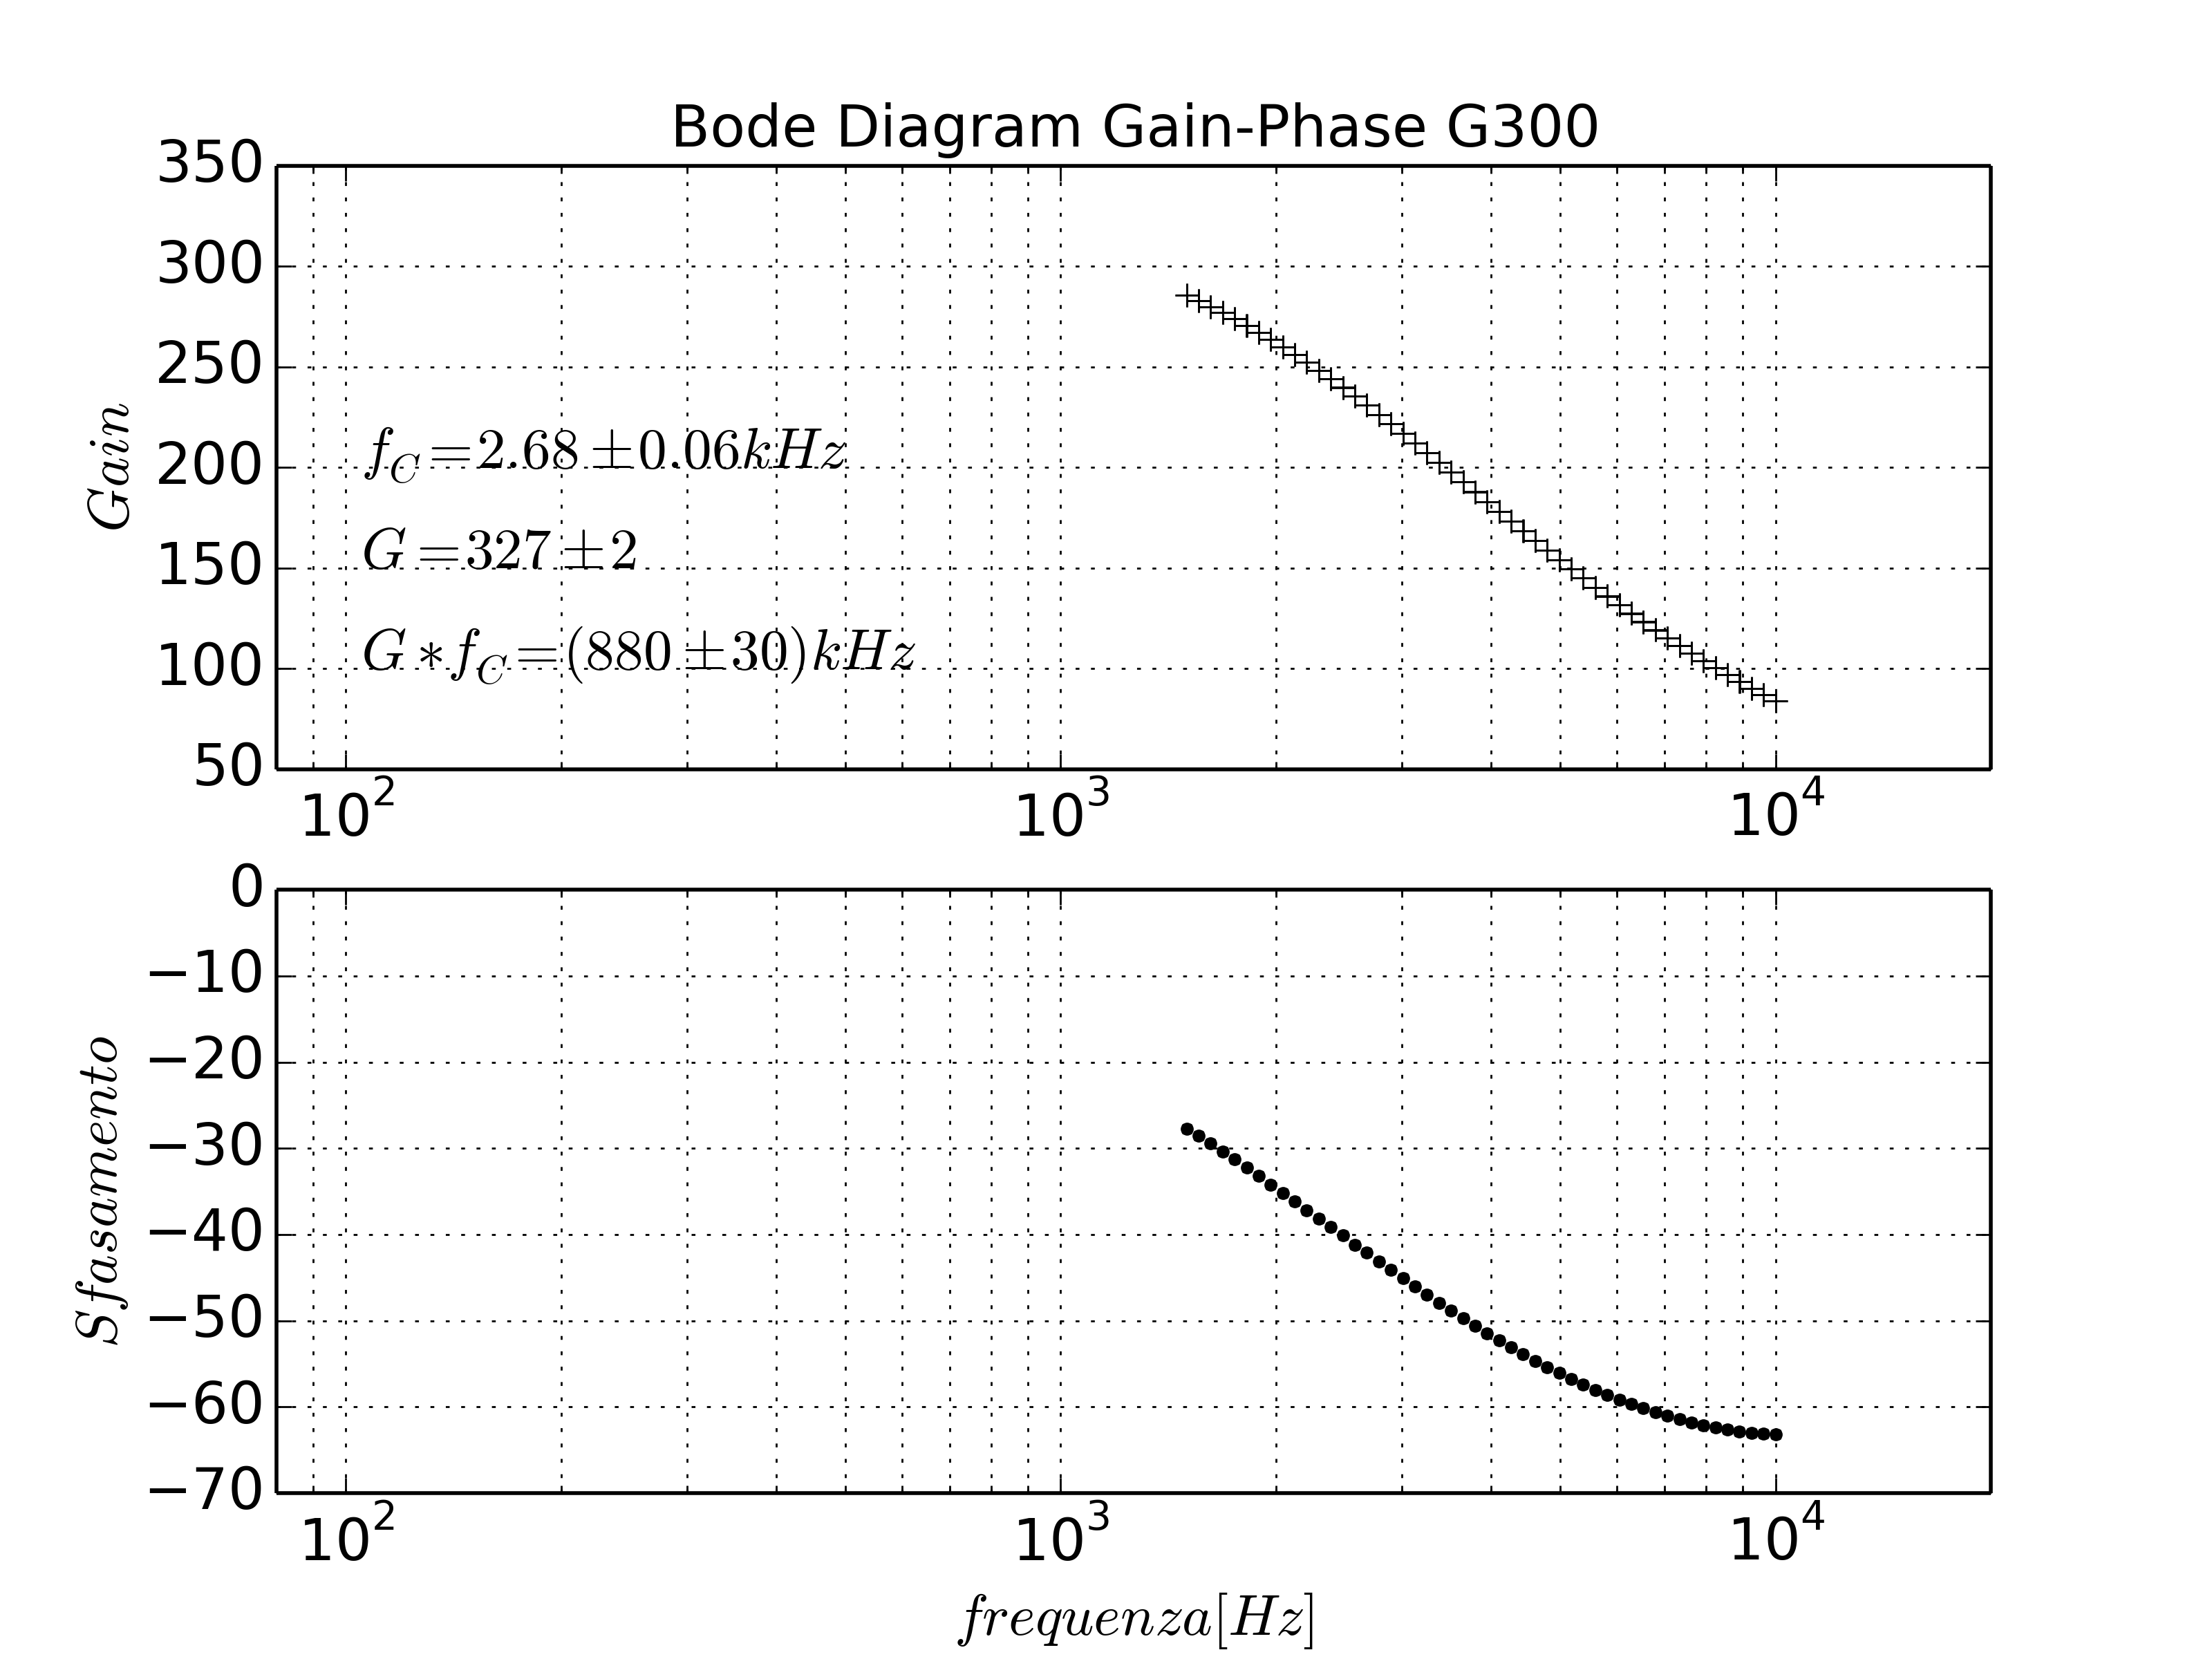
\includegraphics[width=1\linewidth]{./es_9_bode_g300}
\caption{Bode Diagram - G300}
\label{fig:es_9_bode_g300}
\end{figure}
\end{frame}

\begin{frame}

{
\centering
\begin{tabular}{|c|c|}
\hline  &  \textbf{Dati sperimentali G500} \\ 
\hline $R_1$  &  98 \si{Ohm} + 1.03 \si{kOhm} ($\pm$ 0.8 \%) \\ 
\hline $R_2$ & 353 \si{kOhm} + 217  \si{kOhm} $\pm$ 0.8 \%  \\ 
\hline $V_{PP}$ & $ 30  \pm 3 \si{mV} $ \\ 
\hline $V_{OFF} preset$ & $ -46  \si{mV} $ \\
\hline G &  $G_{exp}  = 510 \pm 20  \, G_{meas} = 540 \pm 2 $ \\ 
\hline $f_T (kHz)$ &  1.64 $\pm$ 0.04 \\
\hline $G*f_{T}$ \si{kHz} & $ 880 \pm 30 $\\
\hline
\end{tabular} 

}

\end{frame}

\begin{frame}
\begin{figure}
\centering
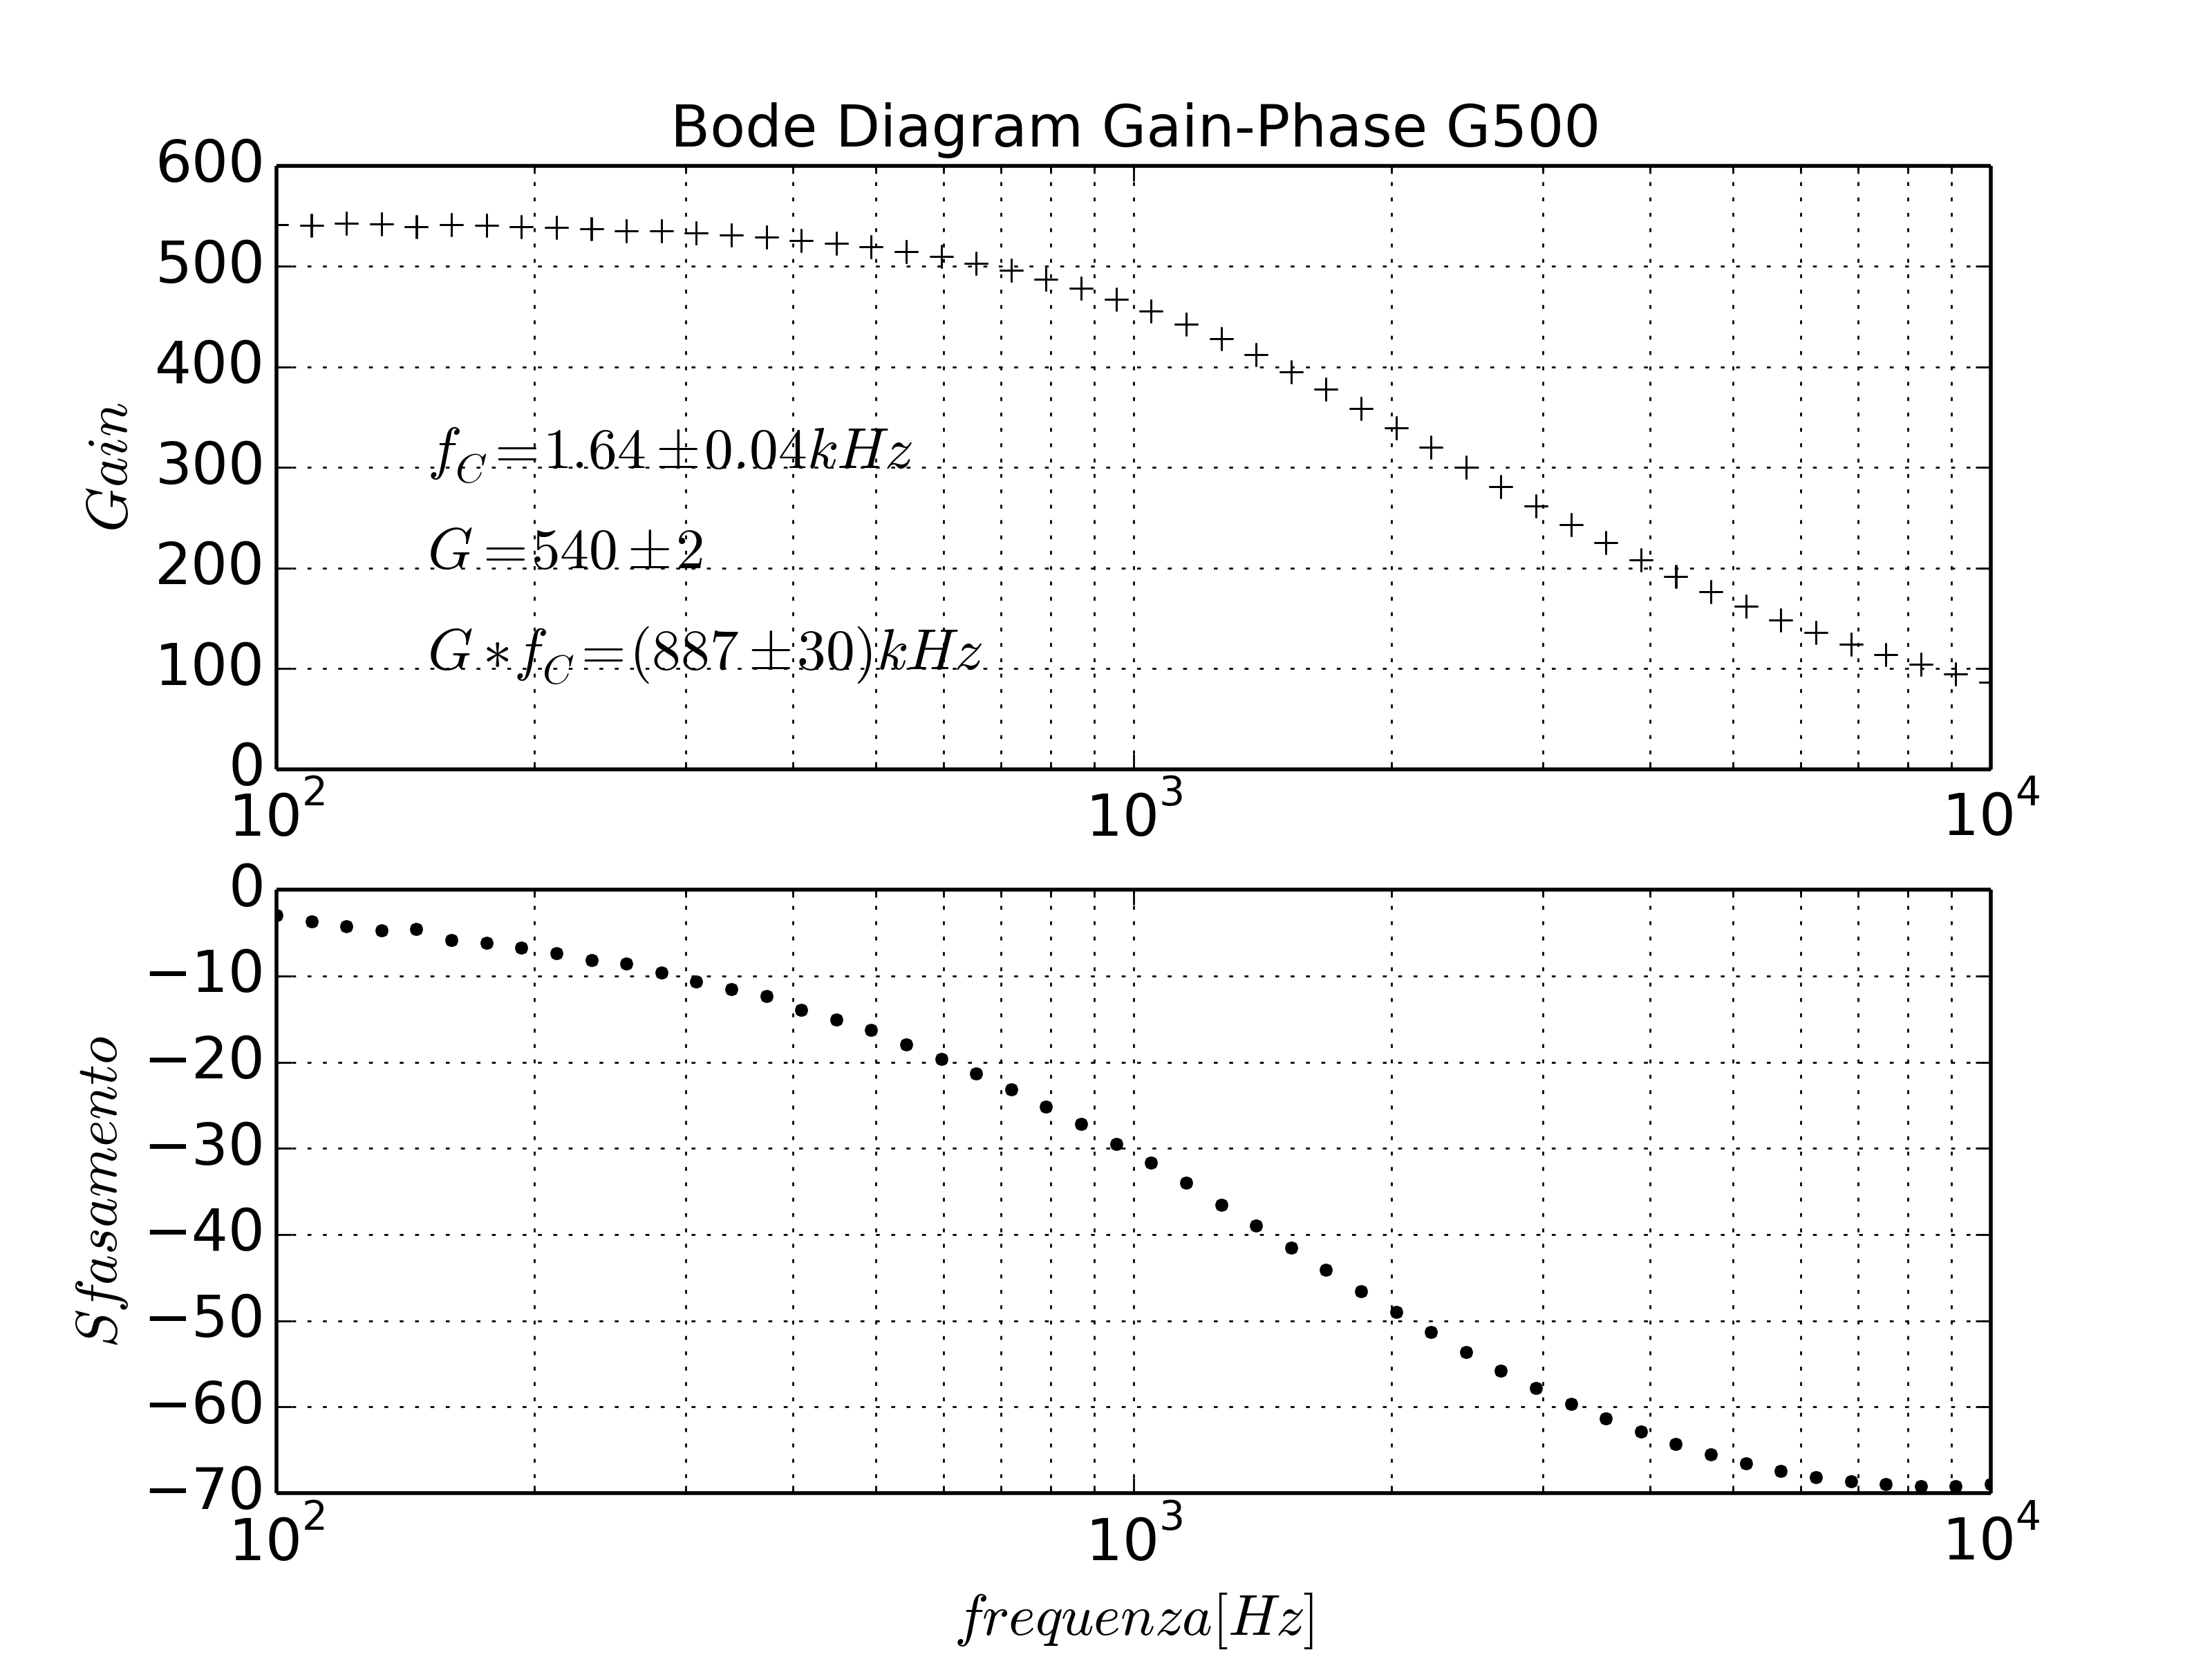
\includegraphics[width=1\linewidth]{./es_9_bode_g500}
\caption{Bode Diagram - G500}
\label{fig:es_9_bode_g500}
\end{figure}

\end{frame}



\begin{frame}{Stima frequenze di taglio per G = 1000, G = 1}

\begin{itemize}
\item A partire dalla relazione $G*f_T = cost$ si ricava:
\end{itemize}

{
\centering
\begin{tabular}{|c|c|}
\hline G & $f_{T}$ \\ 
\hline 1000 &  $850 \si{Hz}$\\ 
\hline 1  &   $8.50 \si{kHz}$ \textbf{\textsc{UGBW}}\\ 
\hline 
\end{tabular}

} 

\begin{itemize}
\item Interpolando graficamente il grafico \textit{OPEN-LOOP LARGE-SIGNAL DIFFERENTIAL VOLTAGE AMPLIFICATION vs
FREQUENCY} riportato sul datasheet del $\mu A741$ si verifica che la frequenza di \textbf{\textsc{UGBW}} è pari circa a $1 \si{MHz}$.
\end{itemize}

\end{frame}

\begin{frame}
\begin{figure}
\centering
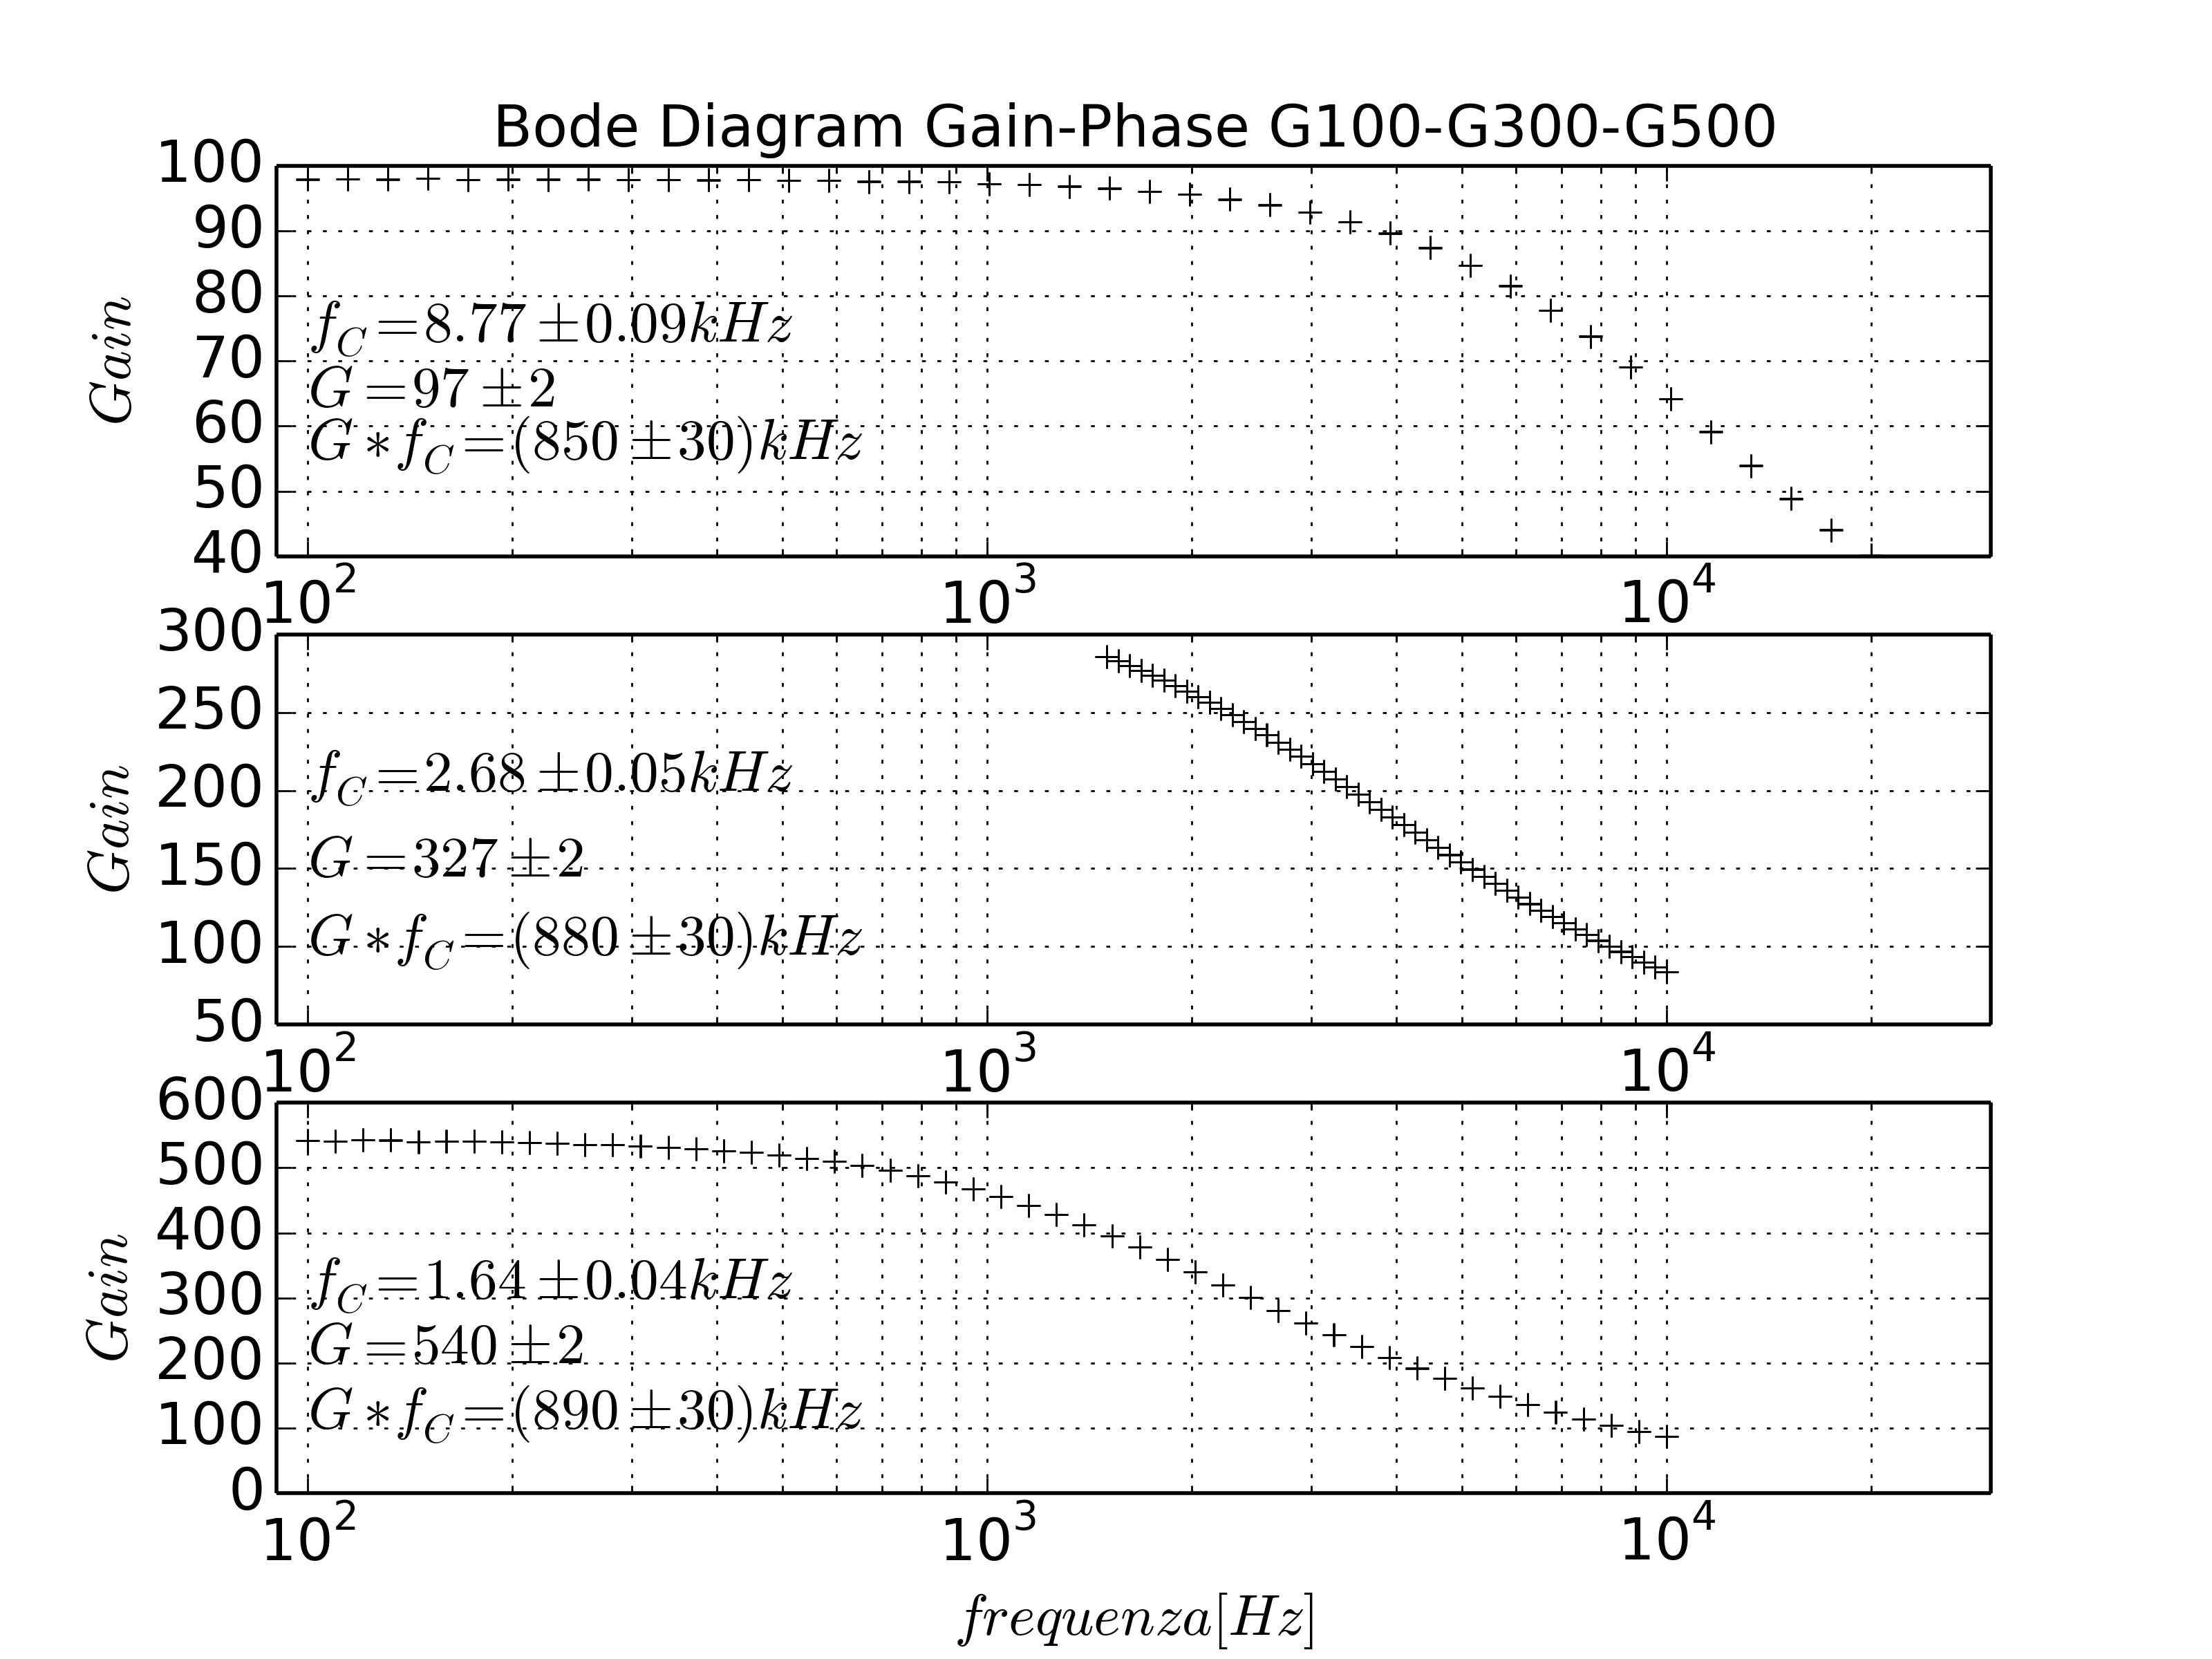
\includegraphics[width=1\linewidth]{./es_9_bode_triplot}
\caption{Triplot Gain 100-300-500 Semilogx}
\label{fig:es_9_bode_triplot}
\end{figure}

\end{frame}

\begin{frame}
\begin{figure}
\centering
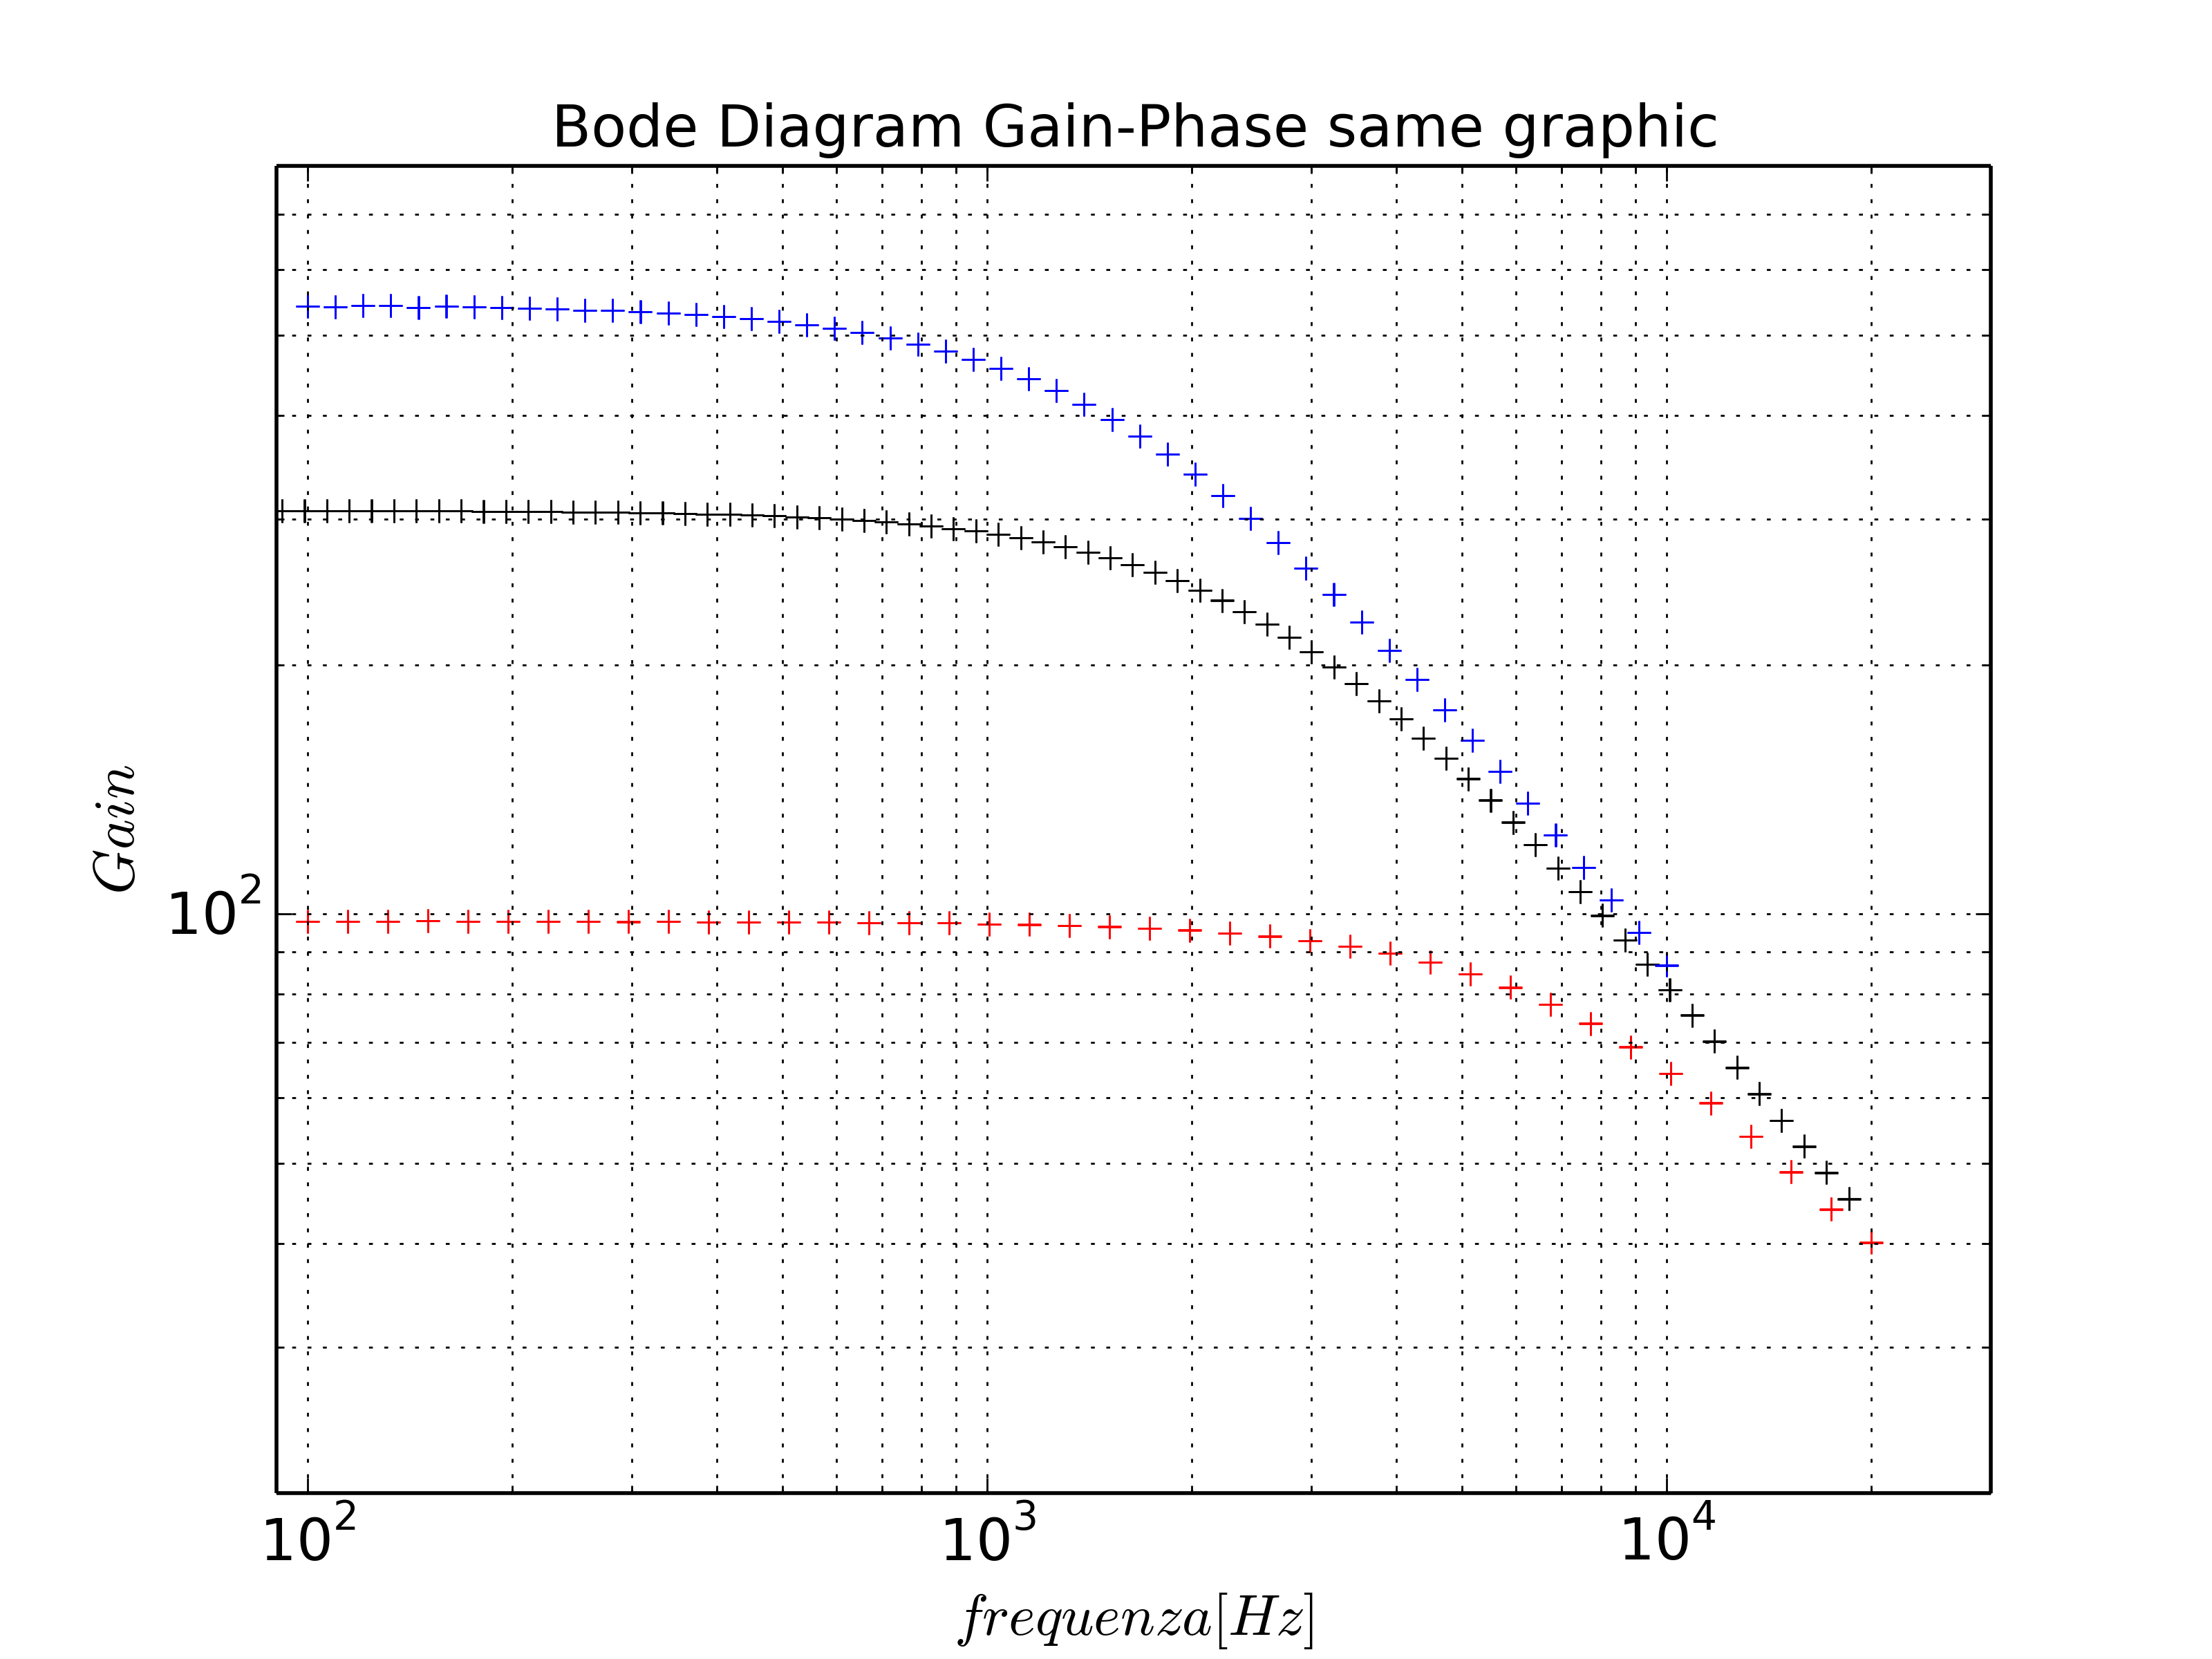
\includegraphics[width=1\linewidth]{./es_9_bode_triplot_same_bilog}
\caption{Bode Diagram - Triplot bilog}
\label{fig:es_9_bode_triplot_same_bilog}
\end{figure}

\end{frame}

% Placing a * after \section means it will not show in the
% outline or table of contents.
\section*{Summary}

\begin{frame}{Summary}
  \begin{itemize}
  \item
    The \alert{first main message} of your talk in one or two lines.
  \item
    The \alert{second main message} of your talk in one or two lines.
  \item
    Perhaps a \alert{third message}, but not more than that.
  \end{itemize}
  
  \begin{itemize}
  \item
    Outlook
    \begin{itemize}
    \item
      Something you haven't solved.
    \item
      Something else you haven't solved.
    \end{itemize}
  \end{itemize}
\end{frame}



% All of the following is optional and typically not needed. 
\appendix
\section<presentation>*{\appendixname}
\subsection<presentation>*{For Further Reading}

\begin{frame}[allowframebreaks]
  \frametitle<presentation>{For Further Reading}
    
  \begin{thebibliography}{10}
    
  \beamertemplatebookbibitems
  % Start with overview books.

  \bibitem{Author1990}
    A.~Author.
    \newblock {\em Handbook of Everything}.
    \newblock Some Press, 1990.
 
    
  \beamertemplatearticlebibitems
  % Followed by interesting articles. Keep the list short. 

  \bibitem{Someone2000}
    S.~Someone.
    \newblock On this and that.
    \newblock {\em Journal of This and That}, 2(1):50--100,
    2000.
  \end{thebibliography}
\end{frame}

\end{document}


